\subsection{Challenges}
\label{subsec:interconnect-sc-dma-challenges}

\subsubsection{Trade-off between small vs large DMA transfers}
\label{subsubsec:interconnect-sc-dma-challenges-trade-off-small-v-large-tx}

Since DMA controllers only provide the completion time of an entire DMA transfer, the adversary faces a trade-off when selecting the transfer size. 
Small transfers enable fine-grained measurements of the presence/absence of victim traffic but cannot saturate a non-hierarchical PCIe link. 
In contrast, large transfers provide coarse-grained measurements but may be able to saturate a non-hierarchical PCIe link, increasing the likelihood of interfering with the victim traffic.
To determine the appropriate transfer size, we profile the execution time and bandwidth utilisation of PCIe across different DMA transfer sizes.

To perform the DMA transfers, we rely on the \textit{cudaMemcpy} function provided by Nvidia CUDA.
We ensure that the memory on the CPU is pinned to the DRAM and can not be swapped, as the DMA controller requires this.
We measure the DMA transfer time using \textit{cudaEventRecord}, which uses a timer from the GPU to measure the time taken by GPU operations such as \textit{cudaMemcpy}
\footnote{While we can follow the approach taken by LockedDown \cite{side2022lockeddown} and use the CPU-side timers such as RDTSC(P), those measurements would include the time taken by the GPU driver to send the transfer information to the DMA controller.}.

% To perform the DMA transfers, we rely on the \textit{cudaMemcpy} function provided by Nvidia CUDA.
% \textit{cudaMemcpy} accepts the source and destination addresses (at least one of which should point to some GPU memory) and the size of the data to be transferred.
% It expects the address associated with the CPU memory (if any) to be pinned in the CPU DRAM (i.e. the memory is not swapped to disk at any point).
% If that is not the case, \textit{cudaMemcpy} first allocates a pinned memory, copies the data over to this memory, and then sends the corresponding commands to the DMA engine for initiating the transfer.

% In our experiments, we rely on memory that is already pinned in the CPU DRAM, thus avoiding the additional overhead of \textit{cudaMemcpy} copying the data to a newly allocated pinned memory.
% In addition, our experiments utilise \textit{cudaEventRecord} provided by CUDA to measure the execution time of \textit{cudaMemcpy}.
% However, \textit{cudaEventRecord} uses the timer from the GPU, which only has a granularity in the order of microseconds.
% In addition, \textit{cudaEventRecord} returns the timer as a floating point number in the order of milliseconds, adding to the inaccuracy of the timer.

As shown in \Cref{fig:bw-util-and-time-per-size}, the transfer time increases with the transfer size, while the transfer rate does not increase beyond 25GBps
\footnote{While the theoretical limit of PCIe 4.0 x16 is 32GBps, the achievable transfer rate is less due to the protocol overheads \cite{neugebauer2018understanding}.},
at a transfer size of 4MB.
Therefore, if an adversary aims to saturate the PCIe bandwidth, they can optimise the transfer size at 4MB to strike a balance between fine-grained measurements and saturating the PCIe bandwidth.

\begin{figure}[!htb]
    \centering
    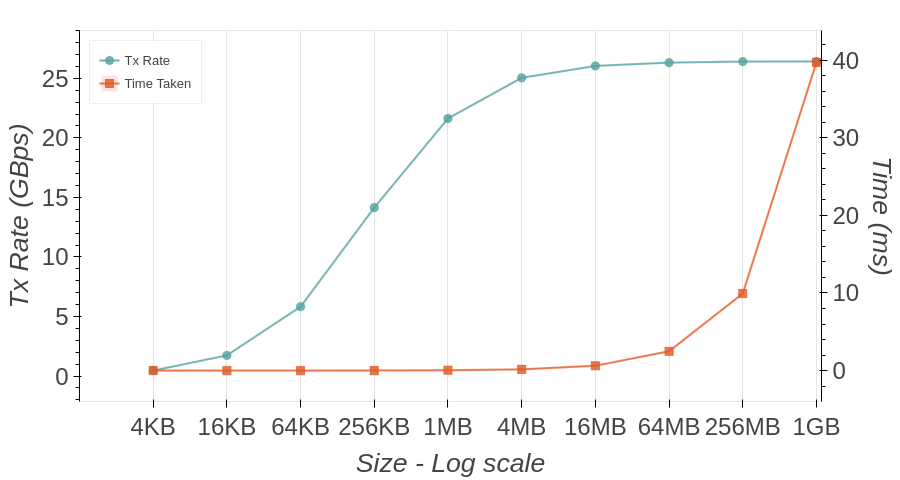
\includegraphics[width=\columnwidth]{figures/interconnect-sc/dma/bw_util_and_time_per_size.png}
    \caption{PCIe bandwidth utilisation and time taken for the DMA transfer}
    \label{fig:bw-util-and-time-per-size}
    % 2025-03-06_16-40
\end{figure}
